\iffalse
\def\mytitle{PARABOLA}                                                            
\def\myauthor{VAMSI SUNKARI}
\def\contact{vamsisunkari9849@gmail.com}
\def\mymodule{Future Wireless Communication (FWC)}
\documentclass[10pt, a4paper]{article}
\usepackage[a4paper,outer=1.5cm,inner=1.5cm,top=1.75cm,bottom=1.5cm]{geometry}
\twocolumn
\usepackage{setspace}
\usepackage{graphicx}
\graphicspath{{./images/}}
\usepackage[colorlinks,linkcolor={black},citecolor={blue!80!black},urlcolor={blue!80!black}]{hyperref}
\usepackage[parfill]{parskip}
\usepackage{lmodern}
\usepackage{tikz}
 \usepackage{physics}
%\documentclass[tikz, border=2mm]{standalone}
\usepackage{karnaugh-map}
\usepackage{tabularx}
\usetikzlibrary{calc}
\usepackage{amsmath}
\usepackage{amssymb}
\renewcommand*\familydefault{\sfdefault}
\usepackage{watermark}
\usepackage{lipsum}
\usepackage{xcolor}
\usepackage{listings}
\usepackage{float}
\usepackage{titlesec}
\providecommand{\mtx}[1]{\mathbf{#1}}
\titlespacing{\subsection}{1pt}{\parskip}{3pt}
\titlespacing{\subsubsection}{0pt}{\parskip}{-\parskip}
\titlespacing{\paragraph}{0pt}{\parskip}{\parskip}
\newcommand{\figuremacro}[5]{//
    \begin{figure}[#1]
        \centering
        \includegraphics[width=#5\columnwidth]{#2}
        \caption[#3]{\textbf{#3}#4}
        \label{fig:#2}
    \end{figure}
}
\newcommand{\myvec}[1]{\ensuremath{\begin{pmatrix}#1\end{pmatrix}}}
\let\vec\mathbf
\lstset{
frame=single,
breaklines=true,
columns=fullflexible
}

\providecommand{\brak}[1]{\ensuremath{\left(#1\right)}}
\providecommand{\lbrak}[1]{\ensuremath{\left(#1\right.}}
\providecommand{\rbrak}[1]{\ensuremath{\left.#1\right)}}
\providecommand{\sbrak}[1]{\ensuremath{{}\left[#1\right]}}
\title{\mytitle}
\author{\myauthor\hspace{1em}\\\contact\\FWC22040\hspace{6.5em}IITH\hspace{0.5em}\mymodule\hspace{6em}ASSIGN-6}
\date{}
\begin{document}
 \maketitle
 \tableofcontents
 \section{Problem}
 \fi
 The line $y=mx+1$ is a tangent to the curve $y^2 = 4x$, find the value of $m$. 
 \\
 \solution 
	\begin{figure}[!h]
		\centering
 \includegraphics[width=\columnwidth]{chapters/12/6/6/21/figs/im.pdf}
		\caption{}
		\label{fig:12/6/6/21}
  	\end{figure}
	\iffalse

\section{Construction}
\includegraphics[width=1\columnwidth]{im.pdf}
\section{Solution}
The equation of parabola is:
\begin{align}
    \vec{X}^T\vec{V}\vec{X} + 2\vec{u}^T\vec{X} + f = 0
\end{align}
\fi
The parameters for the given conic are
\begin{align}
    \vec{V} = \myvec{0&0\\0&1}, \vec{u} = \myvec{-2\\0}, f = 0
		\label{eq:12/6/6/21/param}
\end{align}
The given tangent can be expressed in parametric form as
\begin{align}
		\label{eq:12/6/6/21/tangent}
\vec{x} = \vec{e}_2 + \mu\vec{m}
\end{align}
Substituting from 
		\eqref{eq:12/6/6/21/tangent}
		and
		\eqref{eq:12/6/6/21/param}
		in 
	  \eqref{eq:h-tangents-cond}
and solving, we obtain 
\begin{align}
	m = 1.
\end{align}
\iffalse
Let $\vec{q}$ be the point of contact.   Then, from 
  \eqref{eq:conic_tangent_contact}
\begin{align}
\vec{q}^T\vec{V}\vec{q} + 2\vec{u}^T\vec{q} + f = 0
		\label{eq:12/6/6/21/contact}
\end{align}
Also, from 
  \eqref{eq:conic_tangent_mq},
\begin{align}
    \vec{m}^T(\vec{V}\vec{q}+\vec{u})=0
		\label{eq:12/6/6/21/mp}
\end{align}
From 
		\eqref{eq:12/6/6/21/contact}
		and 
		\eqref{eq:12/6/6/21/mp},


\begin{align}
        \vec{n}^T\vec{q} = 1
\end{align}

By solving,
\begin{align}
        \myvec{-m & 1 \\ 0 & m}\vec{q} = \myvec{1 \\ 2}
\end{align}

The augumented matrix is

\begin{align}
        \myvec{-m & 1 & 1 \\ 0 & m & 2}\xrightarrow[]{R_1 \leftarrow  mR_1 - R_2 } \myvec{-m^2 & 0 & m-2 \\ 0 & m & 2}
\end{align}
\begin{align}
        \vec{q} = \myvec{\frac{2 - m}{m^2} \\ \frac{2}{m}}
\end{align}
Substitute in
\begin{align}
        \vec{q}^T\vec{V}\vec{q} + 2\vec{u}^T\vec{q} + f = 0
\end{align}

\begin{align}
	\myvec{\frac{2 - m}{m^2} & \frac{2}{m}}\myvec{0&0\\0&1}\myvec{\frac{2 - m}{m^2} \\ \frac{2}{m}} + 2\myvec{-2 & 0}\myvec{\frac{2 - m}{m^2} \\ \frac{2}{m}}
\end{align}

\begin{align}
        \frac{4}{m^2} = \frac{4}{m^2} (2 - m)
\end{align}
\begin{align}
        m = 1
\end{align}
\fi
